\section{Discussion}
\label{sec:discussion}

% Downbeat, Downbeat > Downbeat, Upbeat > Upbeat, Upbeat. Combination should use this hierarchy but doesn't really.
% However in combination with the top-down likelihood function it may.
% Expression
% Tempo curves are not relevant anymore. A subdivision approach may be a good way of researching expression in rhythm
% Cognitive plausibility
%	Incremental parsing
%	The bottom-up/top-down estimation of onset times doesn't seem to be very cognitively plausible.
% Other time signatures were not allowed, but theoretically it should be trivial to extend the present method for more time signatures.
% Swing ratio
% Does a pcfg captures temperleys common practice rhythm assumptions
% Combination/observations convoluted
% Not including rests leads to loss of information

\begin{figure}
\subfloat[]{
\parbox{0.5\linewidth}{
\Tree
[ .{$\frac{1}{1}$} [ .{$\frac{1}{2}$} [ .$\bullet$ ] [ .$\bullet$ ] ] [ .{$\frac{1}{2}$} [ .$\bullet$ ] [ .$\bullet$ ] ] ]
}
}
\qquad
\subfloat[]{
\parbox{0.5\linewidth}{
\begin{tabular}{| l  >{\centering\arraybackslash}m{2in} |}
\hline 
A & 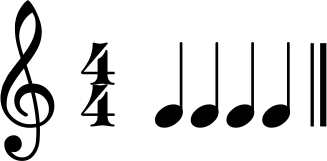
\includegraphics[scale=0.3]{img/discuss1}\\
\hline
\end{tabular}
}
}
\end{figure}

\begin{figure}
\subfloat[]{
\parbox{0.5\linewidth}{
\Tree
[ .{$\frac{1}{1}$} [ .{$\frac{1}{2}$} [ .{$\frac{1}{4}$} [ .$*$ ] [ .$\bullet$ ] ] [ .{$\frac{1}{4}$} [ .$\bullet$ ] [ .$\bullet$ ] ] ] [ .$\bullet$ ] ] 
}
}
\qquad
\subfloat[]{
\parbox{0.5\linewidth}{
\begin{tabular}{| l  >{\centering\arraybackslash}m{2in} |}
\hline 
A & 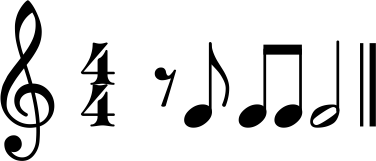
\includegraphics[scale=0.3]{img/discuss2}\\
B & 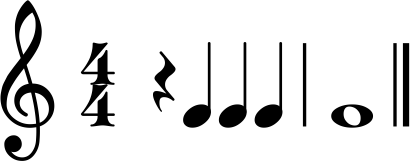
\includegraphics[scale=0.3]{img/discuss3}\\
\hline
\end{tabular}
}
}
\end{figure}

\begin{figure}
\parbox{0.5\linewidth}{
\subfloat[]{
\Tree
[ .{$\frac{1}{1}$} [ .{$\frac{1}{2}$} [ .{$\frac{1}{4}$} [ .$*$ ] [ .$\bullet$ ] ] [ .{$\frac{1}{4}$} [ .$\bullet$ ] [ .$\bullet$ ] ] ] [ .{$\frac{1}{2}$} [ .{$\frac{1}{4}$} [ .$\bullet$ ] [ .Rest ] ] [ .Rest ] ] ]
}
}
\qquad
\subfloat[]{
\parbox{0.5\linewidth}{
\begin{tabular}{| l  >{\centering\arraybackslash}m{2in} |}
\hline 
A & 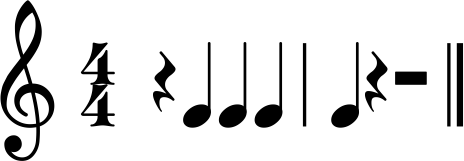
\includegraphics[scale=0.3]{img/discuss4}\\
\hline
\end{tabular}
}
}
\end{figure}

